% Options for packages loaded elsewhere
\PassOptionsToPackage{unicode}{hyperref}
\PassOptionsToPackage{hyphens}{url}
%
\documentclass[
]{article}
\title{MPM.02 Groupwork}
\author{Felix, Regis, Sofie, Philipp}
\date{06/01/2022}

\usepackage{amsmath,amssymb}
\usepackage{lmodern}
\usepackage{iftex}
\ifPDFTeX
  \usepackage[T1]{fontenc}
  \usepackage[utf8]{inputenc}
  \usepackage{textcomp} % provide euro and other symbols
\else % if luatex or xetex
  \usepackage{unicode-math}
  \defaultfontfeatures{Scale=MatchLowercase}
  \defaultfontfeatures[\rmfamily]{Ligatures=TeX,Scale=1}
\fi
% Use upquote if available, for straight quotes in verbatim environments
\IfFileExists{upquote.sty}{\usepackage{upquote}}{}
\IfFileExists{microtype.sty}{% use microtype if available
  \usepackage[]{microtype}
  \UseMicrotypeSet[protrusion]{basicmath} % disable protrusion for tt fonts
}{}
\makeatletter
\@ifundefined{KOMAClassName}{% if non-KOMA class
  \IfFileExists{parskip.sty}{%
    \usepackage{parskip}
  }{% else
    \setlength{\parindent}{0pt}
    \setlength{\parskip}{6pt plus 2pt minus 1pt}}
}{% if KOMA class
  \KOMAoptions{parskip=half}}
\makeatother
\usepackage{xcolor}
\IfFileExists{xurl.sty}{\usepackage{xurl}}{} % add URL line breaks if available
\IfFileExists{bookmark.sty}{\usepackage{bookmark}}{\usepackage{hyperref}}
\hypersetup{
  pdftitle={MPM.02 Groupwork},
  pdfauthor={Felix, Regis, Sofie, Philipp},
  hidelinks,
  pdfcreator={LaTeX via pandoc}}
\urlstyle{same} % disable monospaced font for URLs
\usepackage[margin=1in]{geometry}
\usepackage{color}
\usepackage{fancyvrb}
\newcommand{\VerbBar}{|}
\newcommand{\VERB}{\Verb[commandchars=\\\{\}]}
\DefineVerbatimEnvironment{Highlighting}{Verbatim}{commandchars=\\\{\}}
% Add ',fontsize=\small' for more characters per line
\usepackage{framed}
\definecolor{shadecolor}{RGB}{248,248,248}
\newenvironment{Shaded}{\begin{snugshade}}{\end{snugshade}}
\newcommand{\AlertTok}[1]{\textcolor[rgb]{0.94,0.16,0.16}{#1}}
\newcommand{\AnnotationTok}[1]{\textcolor[rgb]{0.56,0.35,0.01}{\textbf{\textit{#1}}}}
\newcommand{\AttributeTok}[1]{\textcolor[rgb]{0.77,0.63,0.00}{#1}}
\newcommand{\BaseNTok}[1]{\textcolor[rgb]{0.00,0.00,0.81}{#1}}
\newcommand{\BuiltInTok}[1]{#1}
\newcommand{\CharTok}[1]{\textcolor[rgb]{0.31,0.60,0.02}{#1}}
\newcommand{\CommentTok}[1]{\textcolor[rgb]{0.56,0.35,0.01}{\textit{#1}}}
\newcommand{\CommentVarTok}[1]{\textcolor[rgb]{0.56,0.35,0.01}{\textbf{\textit{#1}}}}
\newcommand{\ConstantTok}[1]{\textcolor[rgb]{0.00,0.00,0.00}{#1}}
\newcommand{\ControlFlowTok}[1]{\textcolor[rgb]{0.13,0.29,0.53}{\textbf{#1}}}
\newcommand{\DataTypeTok}[1]{\textcolor[rgb]{0.13,0.29,0.53}{#1}}
\newcommand{\DecValTok}[1]{\textcolor[rgb]{0.00,0.00,0.81}{#1}}
\newcommand{\DocumentationTok}[1]{\textcolor[rgb]{0.56,0.35,0.01}{\textbf{\textit{#1}}}}
\newcommand{\ErrorTok}[1]{\textcolor[rgb]{0.64,0.00,0.00}{\textbf{#1}}}
\newcommand{\ExtensionTok}[1]{#1}
\newcommand{\FloatTok}[1]{\textcolor[rgb]{0.00,0.00,0.81}{#1}}
\newcommand{\FunctionTok}[1]{\textcolor[rgb]{0.00,0.00,0.00}{#1}}
\newcommand{\ImportTok}[1]{#1}
\newcommand{\InformationTok}[1]{\textcolor[rgb]{0.56,0.35,0.01}{\textbf{\textit{#1}}}}
\newcommand{\KeywordTok}[1]{\textcolor[rgb]{0.13,0.29,0.53}{\textbf{#1}}}
\newcommand{\NormalTok}[1]{#1}
\newcommand{\OperatorTok}[1]{\textcolor[rgb]{0.81,0.36,0.00}{\textbf{#1}}}
\newcommand{\OtherTok}[1]{\textcolor[rgb]{0.56,0.35,0.01}{#1}}
\newcommand{\PreprocessorTok}[1]{\textcolor[rgb]{0.56,0.35,0.01}{\textit{#1}}}
\newcommand{\RegionMarkerTok}[1]{#1}
\newcommand{\SpecialCharTok}[1]{\textcolor[rgb]{0.00,0.00,0.00}{#1}}
\newcommand{\SpecialStringTok}[1]{\textcolor[rgb]{0.31,0.60,0.02}{#1}}
\newcommand{\StringTok}[1]{\textcolor[rgb]{0.31,0.60,0.02}{#1}}
\newcommand{\VariableTok}[1]{\textcolor[rgb]{0.00,0.00,0.00}{#1}}
\newcommand{\VerbatimStringTok}[1]{\textcolor[rgb]{0.31,0.60,0.02}{#1}}
\newcommand{\WarningTok}[1]{\textcolor[rgb]{0.56,0.35,0.01}{\textbf{\textit{#1}}}}
\usepackage{graphicx}
\makeatletter
\def\maxwidth{\ifdim\Gin@nat@width>\linewidth\linewidth\else\Gin@nat@width\fi}
\def\maxheight{\ifdim\Gin@nat@height>\textheight\textheight\else\Gin@nat@height\fi}
\makeatother
% Scale images if necessary, so that they will not overflow the page
% margins by default, and it is still possible to overwrite the defaults
% using explicit options in \includegraphics[width, height, ...]{}
\setkeys{Gin}{width=\maxwidth,height=\maxheight,keepaspectratio}
% Set default figure placement to htbp
\makeatletter
\def\fps@figure{htbp}
\makeatother
\setlength{\emergencystretch}{3em} % prevent overfull lines
\providecommand{\tightlist}{%
  \setlength{\itemsep}{0pt}\setlength{\parskip}{0pt}}
\setcounter{secnumdepth}{-\maxdimen} % remove section numbering
\ifLuaTeX
  \usepackage{selnolig}  % disable illegal ligatures
\fi

\begin{document}
\maketitle

{
\setcounter{tocdepth}{4}
\tableofcontents
}
\begin{verbatim}
## Warning: package 'knitr' was built under R version 4.0.5
\end{verbatim}

\begin{verbatim}
## Warning: package 'png' was built under R version 4.0.3
\end{verbatim}

\begin{verbatim}
## Warning: package 'rstudioapi' was built under R version 4.0.3
\end{verbatim}

\begin{verbatim}
## Warning: package 'ggplot2' was built under R version 4.0.5
\end{verbatim}

\begin{verbatim}
## Warning: package 'gridExtra' was built under R version 4.0.5
\end{verbatim}

\begin{verbatim}
## Warning: package 'dplyr' was built under R version 4.0.5
\end{verbatim}

\begin{verbatim}
## 
## Attaching package: 'dplyr'
\end{verbatim}

\begin{verbatim}
## The following object is masked from 'package:gridExtra':
## 
##     combine
\end{verbatim}

\begin{verbatim}
## The following objects are masked from 'package:stats':
## 
##     filter, lag
\end{verbatim}

\begin{verbatim}
## The following objects are masked from 'package:base':
## 
##     intersect, setdiff, setequal, union
\end{verbatim}

\begin{verbatim}
## Warning: package 'caret' was built under R version 4.0.5
\end{verbatim}

\begin{verbatim}
## Loading required package: lattice
\end{verbatim}

\begin{verbatim}
## Warning: package 'lattice' was built under R version 4.0.5
\end{verbatim}

\begin{verbatim}
## Warning: package 'mgcv' was built under R version 4.0.5
\end{verbatim}

\begin{verbatim}
## Loading required package: nlme
\end{verbatim}

\begin{verbatim}
## Warning: package 'nlme' was built under R version 4.0.5
\end{verbatim}

\begin{verbatim}
## 
## Attaching package: 'nlme'
\end{verbatim}

\begin{verbatim}
## The following object is masked from 'package:dplyr':
## 
##     collapse
\end{verbatim}

\begin{verbatim}
## This is mgcv 1.8-38. For overview type 'help("mgcv-package")'.
\end{verbatim}

\begin{verbatim}
## Warning: package 'GGally' was built under R version 4.0.5
\end{verbatim}

\begin{verbatim}
## Registered S3 method overwritten by 'GGally':
##   method from   
##   +.gg   ggplot2
\end{verbatim}

\begin{verbatim}
## Warning: package 'magrittr' was built under R version 4.0.3
\end{verbatim}

\begin{verbatim}
## Warning: package 'mosaicCore' was built under R version 4.0.5
\end{verbatim}

\begin{verbatim}
## 
## Attaching package: 'mosaicCore'
\end{verbatim}

\begin{verbatim}
## The following objects are masked from 'package:dplyr':
## 
##     count, tally
\end{verbatim}

\begin{verbatim}
## Warning: package 'readr' was built under R version 4.0.5
\end{verbatim}

\begin{verbatim}
## Warning: package 'Metrics' was built under R version 4.0.5
\end{verbatim}

\begin{verbatim}
## 
## Attaching package: 'Metrics'
\end{verbatim}

\begin{verbatim}
## The following objects are masked from 'package:caret':
## 
##     precision, recall
\end{verbatim}

\begin{verbatim}
## Warning: package 'data.table' was built under R version 4.0.5
\end{verbatim}

\begin{verbatim}
## 
## Attaching package: 'data.table'
\end{verbatim}

\begin{verbatim}
## The following objects are masked from 'package:dplyr':
## 
##     between, first, last
\end{verbatim}

\begin{verbatim}
## Warning: package 'e1071' was built under R version 4.0.5
\end{verbatim}

\begin{verbatim}
## Warning: package 'kernlab' was built under R version 4.0.3
\end{verbatim}

\begin{verbatim}
## 
## Attaching package: 'kernlab'
\end{verbatim}

\begin{verbatim}
## The following object is masked from 'package:ggplot2':
## 
##     alpha
\end{verbatim}

\begin{verbatim}
## Warning: package 'cowplot' was built under R version 4.0.5
\end{verbatim}

\begin{verbatim}
## Warning: package 'tidyverse' was built under R version 4.0.5
\end{verbatim}

\begin{verbatim}
## -- Attaching packages --------------------------------------- tidyverse 1.3.1 --
\end{verbatim}

\begin{verbatim}
## v tibble  3.1.2     v stringr 1.4.0
## v tidyr   1.1.4     v forcats 0.5.1
## v purrr   0.3.4
\end{verbatim}

\begin{verbatim}
## Warning: package 'tibble' was built under R version 4.0.5
\end{verbatim}

\begin{verbatim}
## Warning: package 'tidyr' was built under R version 4.0.5
\end{verbatim}

\begin{verbatim}
## Warning: package 'purrr' was built under R version 4.0.3
\end{verbatim}

\begin{verbatim}
## Warning: package 'stringr' was built under R version 4.0.3
\end{verbatim}

\begin{verbatim}
## Warning: package 'forcats' was built under R version 4.0.5
\end{verbatim}

\begin{verbatim}
## -- Conflicts ------------------------------------------ tidyverse_conflicts() --
## x kernlab::alpha()      masks ggplot2::alpha()
## x data.table::between() masks dplyr::between()
## x nlme::collapse()      masks dplyr::collapse()
## x dplyr::combine()      masks gridExtra::combine()
## x mosaicCore::count()   masks dplyr::count()
## x purrr::cross()        masks kernlab::cross()
## x tidyr::extract()      masks magrittr::extract()
## x dplyr::filter()       masks stats::filter()
## x data.table::first()   masks dplyr::first()
## x dplyr::lag()          masks stats::lag()
## x data.table::last()    masks dplyr::last()
## x purrr::lift()         masks caret::lift()
## x purrr::set_names()    masks magrittr::set_names()
## x mosaicCore::tally()   masks dplyr::tally()
## x purrr::transpose()    masks data.table::transpose()
\end{verbatim}

\begin{verbatim}
## Warning: package 'neuralnet' was built under R version 4.0.5
\end{verbatim}

\begin{verbatim}
## 
## Attaching package: 'neuralnet'
\end{verbatim}

\begin{verbatim}
## The following object is masked from 'package:dplyr':
## 
##     compute
\end{verbatim}

\#Artificial Neural Network

\#\#Data Preparation \#\#\#Load data

Before starting to create NN models, all categorical variables are
converted into a ``one-hot'' resp. binary variable. This is told to be
best practice, as it should enhance the prediction performance let the
model computing converge faster. Latter is also of great interest due to
the long calculation time of NN models. Also, the dependent variable is
normalized.

\#\#\#Break multi factor variables down into single factor variables

\#\#\#Normalize dependent variable

\#\#ANN Model 1 As a first approach to the data set, a few models are
computed at once with a preset range of layer. A slightly reduced
training data volume is taken (65\%). Each model is five-times cross
validated. Also, the threshold is set to 0.1, which is high error
tolerance value. Those first parameter settings are chosen in order to
compute quantity rather than quality. The result shown below suggests
that there is no need of a third nor a second layer, and that the first
layer doesn't improve with more than four neurons in the first layer.
The Root Mean Square Error is about 183. A prediction-vs-real data plot
provides a visualization of the model performance. This plot suggests
that there might be potential for improvement.

As the output neuron is set with ``linear.output = TRUE'', which means
that the output is a continous number and not a factor.

\#\#\#Split Data into Train and Test Partition

\begin{Shaded}
\begin{Highlighting}[]
\FunctionTok{set.seed}\NormalTok{(}\DecValTok{123}\NormalTok{)}
\NormalTok{indices\_1 }\OtherTok{\textless{}{-}} \FunctionTok{createDataPartition}\NormalTok{(data}\SpecialCharTok{$}\NormalTok{cnt, }\AttributeTok{p=}\NormalTok{.}\DecValTok{65}\NormalTok{, }\AttributeTok{list =}\NormalTok{ F)}
\NormalTok{train\_1 }\OtherTok{\textless{}{-}}\NormalTok{ data }\SpecialCharTok{\%\textgreater{}\%} \FunctionTok{slice}\NormalTok{(indices\_1)}
\NormalTok{test\_1 }\OtherTok{\textless{}{-}}\NormalTok{ data }\SpecialCharTok{\%\textgreater{}\%} \FunctionTok{slice}\NormalTok{(}\SpecialCharTok{{-}}\NormalTok{indices\_1)}
\end{Highlighting}
\end{Shaded}

\#\#\#Set up Parameter Range

\begin{Shaded}
\begin{Highlighting}[]
\FunctionTok{set.seed}\NormalTok{(}\DecValTok{44}\NormalTok{)}
\NormalTok{tuGrid\_1 }\OtherTok{\textless{}{-}} \FunctionTok{expand.grid}\NormalTok{(}\AttributeTok{.layer1=}\FunctionTok{c}\NormalTok{(}\DecValTok{1}\NormalTok{,}\DecValTok{2}\NormalTok{,}\DecValTok{4}\SpecialCharTok{:}\DecValTok{8}\NormalTok{), }\AttributeTok{.layer2=}\FunctionTok{c}\NormalTok{(}\DecValTok{0}\NormalTok{,}\DecValTok{2}\NormalTok{,}\DecValTok{3}\NormalTok{,}\DecValTok{4}\NormalTok{), }\AttributeTok{.layer3=}\FunctionTok{c}\NormalTok{(}\DecValTok{0}\NormalTok{,}\DecValTok{2}\NormalTok{))}
\NormalTok{trCtrl\_1 }\OtherTok{\textless{}{-}} \FunctionTok{trainControl}\NormalTok{(}
  \AttributeTok{method =} \StringTok{\textquotesingle{}repeatedcv\textquotesingle{}}\NormalTok{,}
  \AttributeTok{number =} \DecValTok{5}\NormalTok{,}
  \AttributeTok{repeats =} \DecValTok{1}\NormalTok{,}
  \AttributeTok{returnResamp =} \StringTok{\textquotesingle{}final\textquotesingle{}}\NormalTok{)}
\end{Highlighting}
\end{Shaded}

\#\#\#Train Models

\begin{Shaded}
\begin{Highlighting}[]
\NormalTok{models\_1 }\OtherTok{\textless{}{-}} \FunctionTok{train}\NormalTok{(cnt }\SpecialCharTok{\textasciitilde{}}\NormalTok{ hum }\SpecialCharTok{+}\NormalTok{ temp }\SpecialCharTok{+}\NormalTok{ weathersit\_1 }\SpecialCharTok{+}\NormalTok{ weathersit\_2 }\SpecialCharTok{+}\NormalTok{ weathersit\_3 }\SpecialCharTok{+}\NormalTok{ hr\_1 }\SpecialCharTok{+}\NormalTok{ hr\_2 }\SpecialCharTok{+}\NormalTok{ hr\_3 }\SpecialCharTok{+}\NormalTok{ hr\_4 }\SpecialCharTok{+}\NormalTok{ hr\_5 }\SpecialCharTok{+}\NormalTok{ hr\_6 }\SpecialCharTok{+}\NormalTok{ hr\_7 }\SpecialCharTok{+}\NormalTok{ hr\_8 }\SpecialCharTok{+}\NormalTok{ hr\_9 }\SpecialCharTok{+}\NormalTok{ hr\_10 }\SpecialCharTok{+}\NormalTok{ hr\_11 }\SpecialCharTok{+}\NormalTok{ hr\_12 }\SpecialCharTok{+}\NormalTok{ hr\_13 }\SpecialCharTok{+}\NormalTok{ hr\_14 }\SpecialCharTok{+}\NormalTok{ hr\_15 }\SpecialCharTok{+}\NormalTok{ hr\_16 }\SpecialCharTok{+}\NormalTok{ hr\_17 }\SpecialCharTok{+}\NormalTok{ hr\_18 }\SpecialCharTok{+}\NormalTok{ hr\_19 }\SpecialCharTok{+}\NormalTok{ hr\_20 }\SpecialCharTok{+}\NormalTok{ hr\_21 }\SpecialCharTok{+}\NormalTok{ hr\_22 }\SpecialCharTok{+}\NormalTok{ hr\_23, }\AttributeTok{data =}\NormalTok{ train,}
                  \AttributeTok{method =} \StringTok{\textquotesingle{}neuralnet\textquotesingle{}}\NormalTok{,}
                  \AttributeTok{metric =} \StringTok{\textquotesingle{}RMSE\textquotesingle{}}\NormalTok{,}
                  \AttributeTok{linear.output =} \ConstantTok{TRUE}\NormalTok{,}
                  \AttributeTok{threshold =} \FloatTok{0.1}\NormalTok{,}
                  \AttributeTok{lifesign.step =} \DecValTok{1000}\NormalTok{,}
                  \AttributeTok{lifesign =} \StringTok{"full"}\NormalTok{,}
                  \AttributeTok{preProcess =} \FunctionTok{c}\NormalTok{(}\StringTok{\textquotesingle{}center\textquotesingle{}}\NormalTok{, }\StringTok{\textquotesingle{}scale\textquotesingle{}}\NormalTok{),}
                  \AttributeTok{tuneGrid =}\NormalTok{ tuGrid\_1,}
                  \AttributeTok{trControl =}\NormalTok{ trCtrl\_1)}
\end{Highlighting}
\end{Shaded}

\#\#\#Save resp. Load Model

\begin{Shaded}
\begin{Highlighting}[]
\FunctionTok{saveRDS}\NormalTok{(models\_1, }\StringTok{"neural\_nets\_models\_1.rds"}\NormalTok{)}
\end{Highlighting}
\end{Shaded}

\begin{Shaded}
\begin{Highlighting}[]
\NormalTok{models\_1 }\OtherTok{\textless{}{-}}\FunctionTok{readRDS}\NormalTok{(}\StringTok{"neural\_nets\_models\_1.rds"}\NormalTok{)}
\end{Highlighting}
\end{Shaded}

\#\#\#Plot Models

\begin{Shaded}
\begin{Highlighting}[]
\FunctionTok{plot}\NormalTok{(models\_1)}
\end{Highlighting}
\end{Shaded}

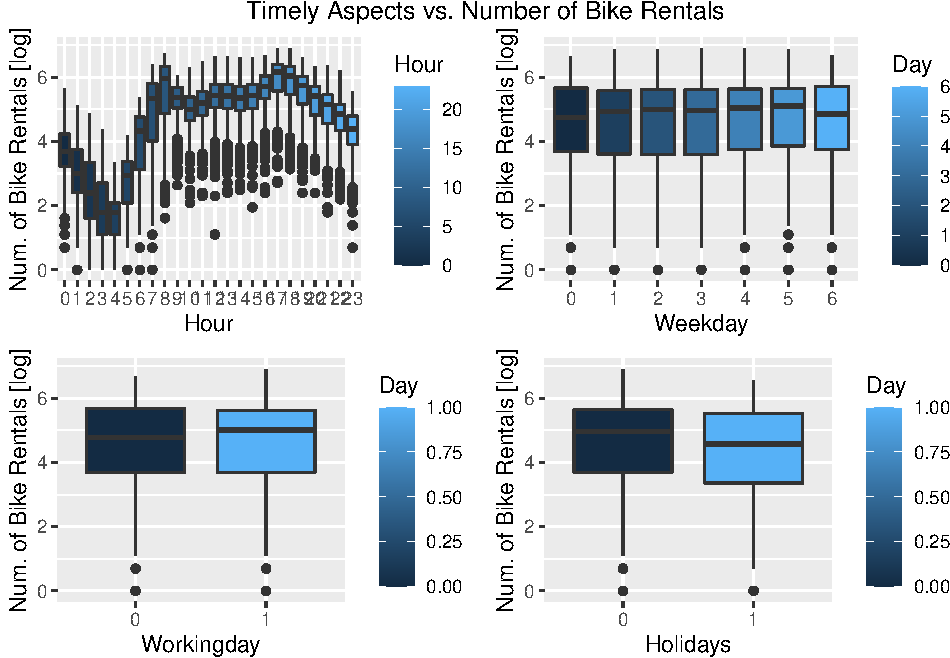
\includegraphics{regis_test_files/figure-latex/unnamed-chunk-10-1.pdf}

\#\#\#Compute Prediction with best Model

\begin{Shaded}
\begin{Highlighting}[]
\NormalTok{pred\_1 }\OtherTok{\textless{}{-}} \FunctionTok{compute}\NormalTok{(models\_1}\SpecialCharTok{$}\NormalTok{finalModel, test\_1 }\SpecialCharTok{\%\textgreater{}\%} \FunctionTok{select}\NormalTok{(}\SpecialCharTok{{-}}\NormalTok{cnt))}
\NormalTok{pred\_1 }\OtherTok{\textless{}{-}}\NormalTok{ pred\_1}\SpecialCharTok{$}\NormalTok{net.result }\SpecialCharTok{*}\NormalTok{ (}\FunctionTok{max}\NormalTok{(df}\SpecialCharTok{$}\NormalTok{cnt) }\SpecialCharTok{{-}} \FunctionTok{min}\NormalTok{(df}\SpecialCharTok{$}\NormalTok{cnt)) }\SpecialCharTok{+} \FunctionTok{min}\NormalTok{(df}\SpecialCharTok{$}\NormalTok{cnt)}
\NormalTok{control\_1 }\OtherTok{\textless{}{-}}\NormalTok{ test\_1}\SpecialCharTok{$}\NormalTok{cnt }\SpecialCharTok{*}\NormalTok{ (}\FunctionTok{max}\NormalTok{(df}\SpecialCharTok{$}\NormalTok{cnt) }\SpecialCharTok{{-}} \FunctionTok{min}\NormalTok{(df}\SpecialCharTok{$}\NormalTok{cnt)) }\SpecialCharTok{+} \FunctionTok{min}\NormalTok{(df}\SpecialCharTok{$}\NormalTok{cnt)}
\end{Highlighting}
\end{Shaded}

\#\#\#Root Mean Square

\begin{Shaded}
\begin{Highlighting}[]
\FunctionTok{sqrt}\NormalTok{(}\FunctionTok{mean}\NormalTok{((control\_1 }\SpecialCharTok{{-}}\NormalTok{ pred\_1)}\SpecialCharTok{\^{}}\DecValTok{2}\NormalTok{))}
\end{Highlighting}
\end{Shaded}

\begin{verbatim}
## [1] 183.5873
\end{verbatim}

\#\#\#Plot Prediction against Real Data

\begin{Shaded}
\begin{Highlighting}[]
\FunctionTok{plot}\NormalTok{(control\_1, pred\_1, }\AttributeTok{col=}\StringTok{\textquotesingle{}orange\textquotesingle{}}\NormalTok{, }\AttributeTok{cex =}\NormalTok{ .}\DecValTok{3}\NormalTok{, }\AttributeTok{pch=}\DecValTok{20}\NormalTok{, }\AttributeTok{ylab =} \StringTok{"predicted rating NN"}\NormalTok{, }\AttributeTok{xlab =} \StringTok{"real rating"}\NormalTok{)}
\FunctionTok{abline}\NormalTok{(}\DecValTok{0}\NormalTok{,}\DecValTok{1}\NormalTok{)}
\end{Highlighting}
\end{Shaded}

\includegraphics{regis_test_files/figure-latex/unnamed-chunk-13-1.pdf}

\#\#ANN Model 2 After the first investigation in the NN layer's
behavior, the four-neurons model layout is taken to be computed again.
This time, a higher data amount (80\%) and an error threshold of 0.01 is
set. The result of this more meticulous model shows already great
improvement in RSME and the plot is also more satisfying. It is unclear
if a model with higher complexity would have performed even better with
a 0.01 threshold, but this is the trade-off for a much faster computing
time.

\#\#\#Split Data into Train and Test Partition

\begin{Shaded}
\begin{Highlighting}[]
\FunctionTok{set.seed}\NormalTok{(}\DecValTok{42}\NormalTok{)}
\NormalTok{indices\_2 }\OtherTok{\textless{}{-}} \FunctionTok{createDataPartition}\NormalTok{(data}\SpecialCharTok{$}\NormalTok{cnt, }\AttributeTok{p=}\NormalTok{.}\DecValTok{8}\NormalTok{, }\AttributeTok{list =}\NormalTok{ F)}

\NormalTok{train\_2 }\OtherTok{\textless{}{-}}\NormalTok{ data }\SpecialCharTok{\%\textgreater{}\%} \FunctionTok{slice}\NormalTok{(indices\_2)}
\NormalTok{test\_2 }\OtherTok{\textless{}{-}}\NormalTok{ data }\SpecialCharTok{\%\textgreater{}\%} \FunctionTok{slice}\NormalTok{(}\SpecialCharTok{{-}}\NormalTok{indices\_2)}
\end{Highlighting}
\end{Shaded}

\#\#\#Train Model

\begin{Shaded}
\begin{Highlighting}[]
\FunctionTok{set.seed}\NormalTok{(}\DecValTok{42}\NormalTok{)}
\NormalTok{model\_2 }\OtherTok{=} \FunctionTok{neuralnet}\NormalTok{(cnt }\SpecialCharTok{\textasciitilde{}}\NormalTok{ hum }\SpecialCharTok{+}\NormalTok{ temp }\SpecialCharTok{+}\NormalTok{ weathersit\_1 }\SpecialCharTok{+}\NormalTok{ weathersit\_2 }\SpecialCharTok{+}\NormalTok{ weathersit\_3 }\SpecialCharTok{+}\NormalTok{ hr\_1 }\SpecialCharTok{+}\NormalTok{ hr\_2 }\SpecialCharTok{+}\NormalTok{ hr\_3 }\SpecialCharTok{+}\NormalTok{ hr\_4 }\SpecialCharTok{+}\NormalTok{ hr\_5 }\SpecialCharTok{+}\NormalTok{ hr\_6 }\SpecialCharTok{+}\NormalTok{ hr\_7 }\SpecialCharTok{+}\NormalTok{ hr\_8 }\SpecialCharTok{+}\NormalTok{ hr\_9 }\SpecialCharTok{+}\NormalTok{ hr\_10 }\SpecialCharTok{+}\NormalTok{ hr\_11 }\SpecialCharTok{+}\NormalTok{ hr\_12 }\SpecialCharTok{+}\NormalTok{ hr\_13 }\SpecialCharTok{+}\NormalTok{ hr\_14 }\SpecialCharTok{+}\NormalTok{ hr\_15 }\SpecialCharTok{+}\NormalTok{ hr\_16 }\SpecialCharTok{+}\NormalTok{ hr\_17 }\SpecialCharTok{+}\NormalTok{ hr\_18 }\SpecialCharTok{+}\NormalTok{ hr\_19 }\SpecialCharTok{+}\NormalTok{ hr\_20 }\SpecialCharTok{+}\NormalTok{ hr\_21 }\SpecialCharTok{+}\NormalTok{ hr\_22 }\SpecialCharTok{+}\NormalTok{ hr\_23, }\AttributeTok{data =}\NormalTok{ train\_2, }\AttributeTok{hidden =} \DecValTok{4}\NormalTok{,}\AttributeTok{linear.output =} \ConstantTok{TRUE}\NormalTok{, }\AttributeTok{threshold =} \FloatTok{0.01}\NormalTok{, }\AttributeTok{stepmax =} \DecValTok{500000}\NormalTok{, }\AttributeTok{lifesign.step =} \DecValTok{1000}\NormalTok{, }\AttributeTok{lifesign =} \StringTok{"full"}\NormalTok{)}
\end{Highlighting}
\end{Shaded}

\#\#\#Save resp. Load Model

\begin{Shaded}
\begin{Highlighting}[]
\FunctionTok{saveRDS}\NormalTok{(model\_2, }\StringTok{"neural\_nets\_model\_2.rds"}\NormalTok{)}
\end{Highlighting}
\end{Shaded}

\begin{Shaded}
\begin{Highlighting}[]
\NormalTok{model\_2 }\OtherTok{\textless{}{-}}\FunctionTok{readRDS}\NormalTok{(}\StringTok{"neural\_nets\_model\_2.rds"}\NormalTok{)}
\end{Highlighting}
\end{Shaded}

\#\#\#Compute Prediction

\begin{Shaded}
\begin{Highlighting}[]
\NormalTok{pred\_2 }\OtherTok{\textless{}{-}} \FunctionTok{compute}\NormalTok{(model\_2, test\_2 }\SpecialCharTok{\%\textgreater{}\%} \FunctionTok{select}\NormalTok{(}\SpecialCharTok{{-}}\NormalTok{cnt))}
\NormalTok{pred\_2 }\OtherTok{\textless{}{-}}\NormalTok{ pred\_2}\SpecialCharTok{$}\NormalTok{net.result }\SpecialCharTok{*}\NormalTok{ (}\FunctionTok{max}\NormalTok{(df}\SpecialCharTok{$}\NormalTok{cnt) }\SpecialCharTok{{-}} \FunctionTok{min}\NormalTok{(df}\SpecialCharTok{$}\NormalTok{cnt)) }\SpecialCharTok{+} \FunctionTok{min}\NormalTok{(df}\SpecialCharTok{$}\NormalTok{cnt)}
\NormalTok{control\_2 }\OtherTok{\textless{}{-}}\NormalTok{ test\_2}\SpecialCharTok{$}\NormalTok{cnt }\SpecialCharTok{*}\NormalTok{ (}\FunctionTok{max}\NormalTok{(df}\SpecialCharTok{$}\NormalTok{cnt) }\SpecialCharTok{{-}} \FunctionTok{min}\NormalTok{(df}\SpecialCharTok{$}\NormalTok{cnt)) }\SpecialCharTok{+} \FunctionTok{min}\NormalTok{(df}\SpecialCharTok{$}\NormalTok{cnt)}
\end{Highlighting}
\end{Shaded}

\#\#\#Root Mean Square

\begin{Shaded}
\begin{Highlighting}[]
\FunctionTok{sqrt}\NormalTok{(}\FunctionTok{mean}\NormalTok{((control\_2 }\SpecialCharTok{{-}}\NormalTok{ pred\_2)}\SpecialCharTok{\^{}}\DecValTok{2}\NormalTok{))}
\end{Highlighting}
\end{Shaded}

\begin{verbatim}
## [1] 100.7022
\end{verbatim}

\#\#\#Plot Prediction against Real Data

\begin{Shaded}
\begin{Highlighting}[]
\FunctionTok{plot}\NormalTok{(control\_2, pred\_2, }\AttributeTok{col=}\StringTok{\textquotesingle{}orange\textquotesingle{}}\NormalTok{, }\AttributeTok{cex =}\NormalTok{ .}\DecValTok{3}\NormalTok{, }\AttributeTok{pch=}\DecValTok{20}\NormalTok{, }\AttributeTok{ylab =} \StringTok{"predicted rating NN"}\NormalTok{, }\AttributeTok{xlab =} \StringTok{"real rating"}\NormalTok{)}
\FunctionTok{abline}\NormalTok{(}\DecValTok{0}\NormalTok{,}\DecValTok{1}\NormalTok{)}
\end{Highlighting}
\end{Shaded}

\includegraphics{regis_test_files/figure-latex/unnamed-chunk-20-1.pdf}

\#\#ANN Model 4: more Predictors, Layer 4/0/0, Threshold 0.05 Now more
predictors are added to the model; the weekdays, the months and the wind
speed. Again with a four-neuron model, the model is computed with a
threshold of 0.05. The results shows improvement in RSME (77) and thus
suggest that there is valuable information in the added predictors.
Again, the plot appear to be better.

\#\#\#Train Model

\begin{Shaded}
\begin{Highlighting}[]
\FunctionTok{set.seed}\NormalTok{(}\DecValTok{41}\NormalTok{)}
\NormalTok{model\_4 }\OtherTok{=} \FunctionTok{neuralnet}\NormalTok{(cnt }\SpecialCharTok{\textasciitilde{}}\NormalTok{ hum }\SpecialCharTok{+}\NormalTok{ temp }\SpecialCharTok{+}\NormalTok{ windspeed }\SpecialCharTok{+}\NormalTok{ weathersit\_1 }\SpecialCharTok{+}\NormalTok{ weathersit\_2 }\SpecialCharTok{+}\NormalTok{ weathersit\_3 }\SpecialCharTok{+}\NormalTok{ hr\_1 }\SpecialCharTok{+}\NormalTok{ hr\_2 }\SpecialCharTok{+}\NormalTok{ hr\_3 }\SpecialCharTok{+}\NormalTok{ hr\_4 }\SpecialCharTok{+}\NormalTok{ hr\_5 }\SpecialCharTok{+}\NormalTok{ hr\_6 }\SpecialCharTok{+}\NormalTok{ hr\_7 }\SpecialCharTok{+}\NormalTok{ hr\_8 }\SpecialCharTok{+}\NormalTok{ hr\_9 }\SpecialCharTok{+}\NormalTok{ hr\_10 }\SpecialCharTok{+}\NormalTok{ hr\_11 }\SpecialCharTok{+}\NormalTok{ hr\_12 }\SpecialCharTok{+}\NormalTok{ hr\_13 }\SpecialCharTok{+}\NormalTok{ hr\_14 }\SpecialCharTok{+}\NormalTok{ hr\_15 }\SpecialCharTok{+}\NormalTok{ hr\_16 }\SpecialCharTok{+}\NormalTok{ hr\_17 }\SpecialCharTok{+}\NormalTok{ hr\_18 }\SpecialCharTok{+}\NormalTok{ hr\_19 }\SpecialCharTok{+}\NormalTok{ hr\_20 }\SpecialCharTok{+}\NormalTok{ hr\_21 }\SpecialCharTok{+}\NormalTok{ hr\_22 }\SpecialCharTok{+}\NormalTok{ hr\_23 }\SpecialCharTok{+}\NormalTok{ weekday\_1 }\SpecialCharTok{+}\NormalTok{ weekday\_2 }\SpecialCharTok{+}\NormalTok{ weekday\_3 }\SpecialCharTok{+}\NormalTok{ weekday\_4 }\SpecialCharTok{+}\NormalTok{ weekday\_5 }\SpecialCharTok{+}\NormalTok{ weekday\_6 }\SpecialCharTok{+}\NormalTok{ weekday\_7 }\SpecialCharTok{+}\NormalTok{ mnth\_1 }\SpecialCharTok{+}\NormalTok{ mnth\_2 }\SpecialCharTok{+}\NormalTok{ mnth\_3 }\SpecialCharTok{+}\NormalTok{ mnth\_4 }\SpecialCharTok{+}\NormalTok{ mnth\_5 }\SpecialCharTok{+}\NormalTok{ mnth\_6 }\SpecialCharTok{+}\NormalTok{ mnth\_7 }\SpecialCharTok{+}\NormalTok{ mnth\_8 }\SpecialCharTok{+}\NormalTok{ mnth\_9 }\SpecialCharTok{+}\NormalTok{ mnth\_10 }\SpecialCharTok{+}\NormalTok{ mnth\_11 }\SpecialCharTok{+}\NormalTok{ mnth\_12, }\AttributeTok{data =}\NormalTok{ train\_2, }\AttributeTok{hidden =} \FunctionTok{c}\NormalTok{(}\DecValTok{4}\NormalTok{),}\AttributeTok{linear.output =} \ConstantTok{TRUE}\NormalTok{, }\AttributeTok{threshold =} \FloatTok{0.05}\NormalTok{, }\AttributeTok{stepmax =} \DecValTok{600000}\NormalTok{, }\AttributeTok{lifesign.step =} \DecValTok{1000}\NormalTok{, }\AttributeTok{lifesign =} \StringTok{"full"}\NormalTok{)}
\end{Highlighting}
\end{Shaded}

\#\#\#Load model (computed in advance)

\begin{Shaded}
\begin{Highlighting}[]
\NormalTok{model\_4 }\OtherTok{\textless{}{-}}\FunctionTok{readRDS}\NormalTok{(}\StringTok{"neural\_nets\_model\_4.rds"}\NormalTok{)}
\end{Highlighting}
\end{Shaded}

\#\#\#Compute Prediction

\#\#\#Root Mean Square

\begin{verbatim}
## [1] 77.30468
\end{verbatim}

\#\#\#Plot Model Performance
\includegraphics{regis_test_files/figure-latex/unnamed-chunk-25-1.pdf}

confidence.interval(x, alpha = 0.05)

confidence.interval(model)

gwplot(x, rep = NULL, max = NULL, min = NULL, file = NULL,
selected.covariate = 1, selected.response = 1, highlight = FALSE, type =
``p'', col = ``black'', \ldots)

gwplot(net.infert, selected.covariate=``parity'') gwplot(net.infert,
selected.covariate=``induced'') gwplot(net.infert,
selected.covariate=``spontaneous'')

\#\#ANN Models 5 With the new predictors added, the model might benefit
from a new layer architecture. Again, a range of model is computed. But
this time, more data (80\%) and new predictors are added. The result
suggest a model architecture of 7,3,0 neurons.

\#\#\#Set up Parameter Range

\begin{Shaded}
\begin{Highlighting}[]
\FunctionTok{set.seed}\NormalTok{(}\DecValTok{44}\NormalTok{)}
\NormalTok{tuGrid\_2 }\OtherTok{\textless{}{-}} \FunctionTok{expand.grid}\NormalTok{(}\AttributeTok{.layer1=}\FunctionTok{c}\NormalTok{(}\DecValTok{4}\SpecialCharTok{:}\DecValTok{8}\NormalTok{), }\AttributeTok{.layer2=}\FunctionTok{c}\NormalTok{(}\DecValTok{0}\NormalTok{,}\DecValTok{2}\NormalTok{,}\DecValTok{3}\NormalTok{,}\DecValTok{4}\NormalTok{), }\AttributeTok{.layer3=}\FunctionTok{c}\NormalTok{(}\DecValTok{0}\NormalTok{,}\DecValTok{2}\NormalTok{))}

\NormalTok{trCtrl\_2 }\OtherTok{\textless{}{-}} \FunctionTok{trainControl}\NormalTok{(}
  \AttributeTok{method =} \StringTok{\textquotesingle{}repeatedcv\textquotesingle{}}\NormalTok{,}
  \AttributeTok{number =} \DecValTok{5}\NormalTok{,}
  \AttributeTok{repeats =} \DecValTok{1}\NormalTok{,}
  \AttributeTok{returnResamp =} \StringTok{\textquotesingle{}final\textquotesingle{}}\NormalTok{,}
\NormalTok{)}
\end{Highlighting}
\end{Shaded}

\#\#\#Train Models

\begin{Shaded}
\begin{Highlighting}[]
\NormalTok{models\_5 }\OtherTok{\textless{}{-}} \FunctionTok{train}\NormalTok{(cnt }\SpecialCharTok{\textasciitilde{}}\NormalTok{ hum }\SpecialCharTok{+}\NormalTok{ temp }\SpecialCharTok{+}\NormalTok{ windspeed }\SpecialCharTok{+}\NormalTok{ weathersit\_1 }\SpecialCharTok{+}\NormalTok{ weathersit\_2 }\SpecialCharTok{+}\NormalTok{ weathersit\_3 }\SpecialCharTok{+}\NormalTok{ hr\_1 }\SpecialCharTok{+}\NormalTok{ hr\_2 }\SpecialCharTok{+}\NormalTok{ hr\_3 }\SpecialCharTok{+}\NormalTok{ hr\_4 }\SpecialCharTok{+}\NormalTok{ hr\_5 }\SpecialCharTok{+}\NormalTok{ hr\_6 }\SpecialCharTok{+}\NormalTok{ hr\_7 }\SpecialCharTok{+}\NormalTok{ hr\_8 }\SpecialCharTok{+}\NormalTok{ hr\_9 }\SpecialCharTok{+}\NormalTok{ hr\_10 }\SpecialCharTok{+}\NormalTok{ hr\_11 }\SpecialCharTok{+}\NormalTok{ hr\_12 }\SpecialCharTok{+}\NormalTok{ hr\_13 }\SpecialCharTok{+}\NormalTok{ hr\_14 }\SpecialCharTok{+}\NormalTok{ hr\_15 }\SpecialCharTok{+}\NormalTok{ hr\_16 }\SpecialCharTok{+}\NormalTok{ hr\_17 }\SpecialCharTok{+}\NormalTok{ hr\_18 }\SpecialCharTok{+}\NormalTok{ hr\_19 }\SpecialCharTok{+}\NormalTok{ hr\_20 }\SpecialCharTok{+}\NormalTok{ hr\_21 }\SpecialCharTok{+}\NormalTok{ hr\_22 }\SpecialCharTok{+}\NormalTok{ hr\_23 }\SpecialCharTok{+}\NormalTok{ weekday\_1 }\SpecialCharTok{+}\NormalTok{ weekday\_2 }\SpecialCharTok{+}\NormalTok{ weekday\_3 }\SpecialCharTok{+}\NormalTok{ weekday\_4 }\SpecialCharTok{+}\NormalTok{ weekday\_5 }\SpecialCharTok{+}\NormalTok{ weekday\_6 }\SpecialCharTok{+}\NormalTok{ weekday\_7 }\SpecialCharTok{+}\NormalTok{ mnth\_1 }\SpecialCharTok{+}\NormalTok{ mnth\_2 }\SpecialCharTok{+}\NormalTok{ mnth\_3 }\SpecialCharTok{+}\NormalTok{ mnth\_4 }\SpecialCharTok{+}\NormalTok{ mnth\_5 }\SpecialCharTok{+}\NormalTok{ mnth\_6 }\SpecialCharTok{+}\NormalTok{ mnth\_7 }\SpecialCharTok{+}\NormalTok{ mnth\_8 }\SpecialCharTok{+}\NormalTok{ mnth\_9 }\SpecialCharTok{+}\NormalTok{ mnth\_10 }\SpecialCharTok{+}\NormalTok{ mnth\_11 }\SpecialCharTok{+}\NormalTok{ mnth\_12, }\AttributeTok{data =}\NormalTok{ train\_2,}
  \AttributeTok{method =} \StringTok{\textquotesingle{}neuralnet\textquotesingle{}}\NormalTok{,}
  \AttributeTok{metric =} \StringTok{\textquotesingle{}RMSE\textquotesingle{}}\NormalTok{,}
  \AttributeTok{linear.output =} \ConstantTok{TRUE}\NormalTok{,}
  \AttributeTok{threshold =} \FloatTok{0.1}\NormalTok{,}
  \AttributeTok{stepmax =} \DecValTok{250000}\NormalTok{,}
  \AttributeTok{lifesign.step =} \DecValTok{1000}\NormalTok{,}
  \AttributeTok{lifesign =} \StringTok{"full"}\NormalTok{,}
  \AttributeTok{preProcess =} \FunctionTok{c}\NormalTok{(}\StringTok{\textquotesingle{}center\textquotesingle{}}\NormalTok{, }\StringTok{\textquotesingle{}scale\textquotesingle{}}\NormalTok{),}
  \AttributeTok{tuneGrid =}\NormalTok{ tuGrid\_2,}
  \AttributeTok{trControl =}\NormalTok{ trCtrl\_2)}
\end{Highlighting}
\end{Shaded}

\#\#\#Plot Models

\begin{Shaded}
\begin{Highlighting}[]
\FunctionTok{plot}\NormalTok{(models\_5)}
\end{Highlighting}
\end{Shaded}

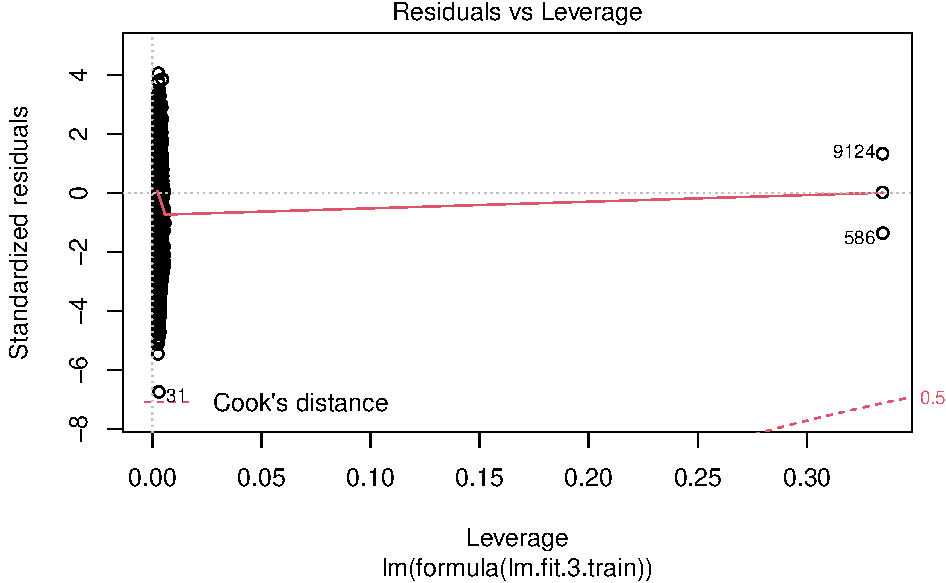
\includegraphics{regis_test_files/figure-latex/unnamed-chunk-29-1.pdf}

\#\#\#Compute Prediction

\begin{Shaded}
\begin{Highlighting}[]
\NormalTok{pred\_5 }\OtherTok{\textless{}{-}} \FunctionTok{compute}\NormalTok{(models\_5}\SpecialCharTok{$}\NormalTok{finalModel, test\_2 }\SpecialCharTok{\%\textgreater{}\%} \FunctionTok{select}\NormalTok{(}\SpecialCharTok{{-}}\NormalTok{cnt))}
\NormalTok{pred\_5 }\OtherTok{\textless{}{-}}\NormalTok{ pred\_5}\SpecialCharTok{$}\NormalTok{net.result }\SpecialCharTok{*}\NormalTok{ (}\FunctionTok{max}\NormalTok{(df}\SpecialCharTok{$}\NormalTok{cnt) }\SpecialCharTok{{-}} \FunctionTok{min}\NormalTok{(df}\SpecialCharTok{$}\NormalTok{cnt)) }\SpecialCharTok{+} \FunctionTok{min}\NormalTok{(df}\SpecialCharTok{$}\NormalTok{cnt)}
\NormalTok{control\_5 }\OtherTok{\textless{}{-}}\NormalTok{ test\_2}\SpecialCharTok{$}\NormalTok{cnt }\SpecialCharTok{*}\NormalTok{ (}\FunctionTok{max}\NormalTok{(df}\SpecialCharTok{$}\NormalTok{cnt) }\SpecialCharTok{{-}} \FunctionTok{min}\NormalTok{(df}\SpecialCharTok{$}\NormalTok{cnt)) }\SpecialCharTok{+} \FunctionTok{min}\NormalTok{(df}\SpecialCharTok{$}\NormalTok{cnt)}
\end{Highlighting}
\end{Shaded}

\#\#\#Root Mean Square

\begin{Shaded}
\begin{Highlighting}[]
\FunctionTok{sqrt}\NormalTok{(}\FunctionTok{mean}\NormalTok{((control\_5 }\SpecialCharTok{{-}}\NormalTok{ pred\_5)}\SpecialCharTok{\^{}}\DecValTok{2}\NormalTok{))}
\end{Highlighting}
\end{Shaded}

\begin{verbatim}
## [1] 238.1291
\end{verbatim}

\#\#\#Plot Prediction against Real Data

\begin{Shaded}
\begin{Highlighting}[]
\FunctionTok{plot}\NormalTok{(control\_5, pred\_5, }\AttributeTok{col=}\StringTok{\textquotesingle{}orange\textquotesingle{}}\NormalTok{, }\AttributeTok{cex =}\NormalTok{ .}\DecValTok{3}\NormalTok{, }\AttributeTok{pch=}\DecValTok{20}\NormalTok{, }\AttributeTok{ylab =} \StringTok{"predicted rating NN"}\NormalTok{, }\AttributeTok{xlab =} \StringTok{"real rating"}\NormalTok{)}
\FunctionTok{abline}\NormalTok{(}\DecValTok{0}\NormalTok{,}\DecValTok{1}\NormalTok{)}
\end{Highlighting}
\end{Shaded}

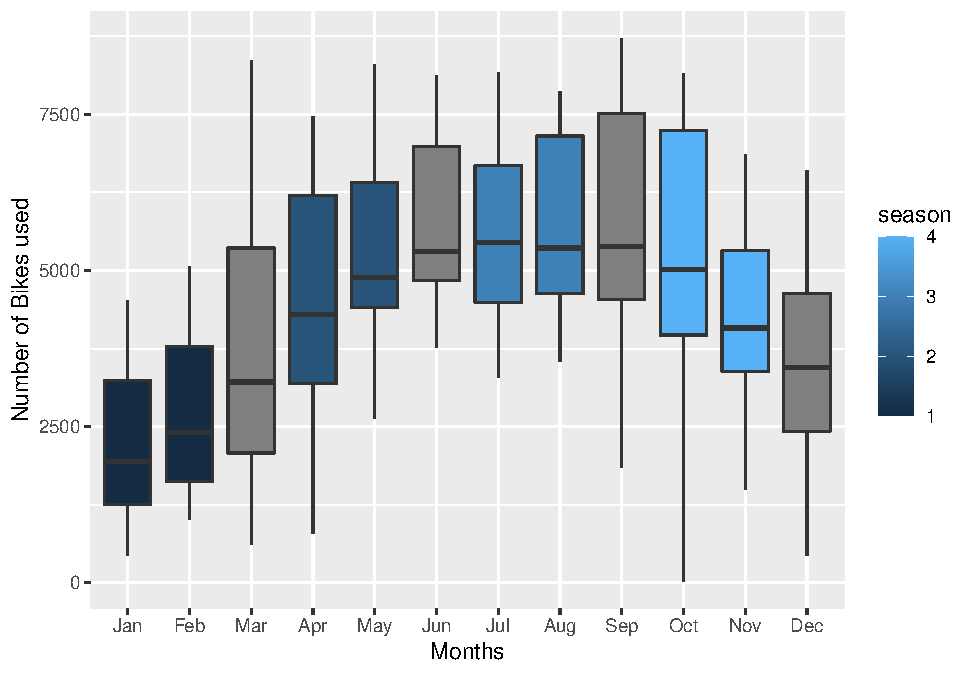
\includegraphics{regis_test_files/figure-latex/unnamed-chunk-32-1.pdf}
\#\#ANN Model 6: Layer 7/3/0, Threshold 0.01 The 7,3,0 model is computed
again but with higher ``resolution''. The RSME drops down to 70.

\#\#\#Compute Prediction

\begin{Shaded}
\begin{Highlighting}[]
\NormalTok{pred\_6 }\OtherTok{\textless{}{-}} \FunctionTok{compute}\NormalTok{(model\_6, test\_2 }\SpecialCharTok{\%\textgreater{}\%} \FunctionTok{select}\NormalTok{(}\SpecialCharTok{{-}}\NormalTok{cnt))}
\NormalTok{pred\_6 }\OtherTok{\textless{}{-}}\NormalTok{ pred\_6}\SpecialCharTok{$}\NormalTok{net.result }\SpecialCharTok{*}\NormalTok{ (}\FunctionTok{max}\NormalTok{(df}\SpecialCharTok{$}\NormalTok{cnt) }\SpecialCharTok{{-}} \FunctionTok{min}\NormalTok{(df}\SpecialCharTok{$}\NormalTok{cnt)) }\SpecialCharTok{+} \FunctionTok{min}\NormalTok{(df}\SpecialCharTok{$}\NormalTok{cnt)}
\NormalTok{control\_6 }\OtherTok{\textless{}{-}}\NormalTok{ test\_2}\SpecialCharTok{$}\NormalTok{cnt }\SpecialCharTok{*}\NormalTok{ (}\FunctionTok{max}\NormalTok{(df}\SpecialCharTok{$}\NormalTok{cnt) }\SpecialCharTok{{-}} \FunctionTok{min}\NormalTok{(df}\SpecialCharTok{$}\NormalTok{cnt)) }\SpecialCharTok{+} \FunctionTok{min}\NormalTok{(df}\SpecialCharTok{$}\NormalTok{cnt)}
\end{Highlighting}
\end{Shaded}

\#\#\#Root Mean Square

\begin{Shaded}
\begin{Highlighting}[]
\FunctionTok{sqrt}\NormalTok{(}\FunctionTok{mean}\NormalTok{((control\_6 }\SpecialCharTok{{-}}\NormalTok{ pred\_6)}\SpecialCharTok{\^{}}\DecValTok{2}\NormalTok{))}
\end{Highlighting}
\end{Shaded}

\begin{verbatim}
## [1] 70.65027
\end{verbatim}

\#\#\#Plot Prediction against Real Data

\begin{Shaded}
\begin{Highlighting}[]
\FunctionTok{plot}\NormalTok{(control\_6, pred\_6, }\AttributeTok{col=}\StringTok{\textquotesingle{}orange\textquotesingle{}}\NormalTok{, }\AttributeTok{cex =}\NormalTok{ .}\DecValTok{3}\NormalTok{, }\AttributeTok{pch=}\DecValTok{20}\NormalTok{, }\AttributeTok{ylab =} \StringTok{"predicted rating NN"}\NormalTok{, }\AttributeTok{xlab =} \StringTok{"real rating"}\NormalTok{)}
\FunctionTok{abline}\NormalTok{(}\DecValTok{0}\NormalTok{,}\DecValTok{1}\NormalTok{)}
\end{Highlighting}
\end{Shaded}

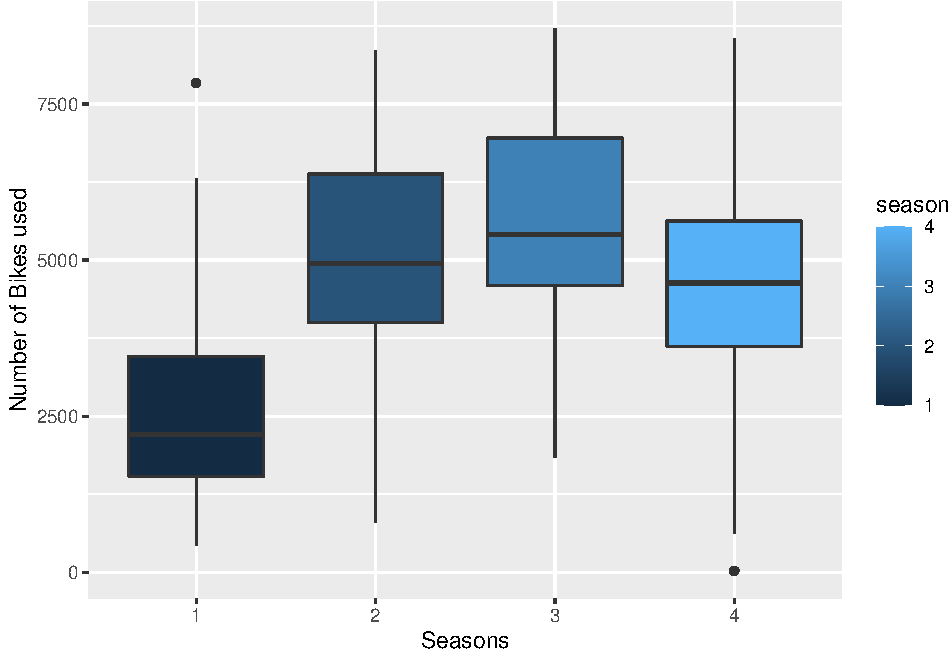
\includegraphics{regis_test_files/figure-latex/unnamed-chunk-37-1.pdf}

\hypertarget{ann-model-9-new-pred.-year-layer-730-threshold-0.01}{%
\subsection{ANN Model 9: New Pred.: Year, Layer 7/3/0, Threshold
0.01}\label{ann-model-9-new-pred.-year-layer-730-threshold-0.01}}

After some reflections about the data, one potential mistake stood out.
Initially, the variable ``year'' was left out, since the data set covers
only two years. But, as there is an increasing trend in the bike rental
over the two years, there might be information in this predictor. The
predictor ``year'' is added to the model 7,3,0. The result shows a great
improvement in RSME with a drop to 49. The plot shows an overall better
prediction behavior.

\begin{Shaded}
\begin{Highlighting}[]
\NormalTok{model\_9 }\OtherTok{\textless{}{-}}\FunctionTok{readRDS}\NormalTok{(}\StringTok{"neural\_nets\_model\_9.rds"}\NormalTok{)}
\end{Highlighting}
\end{Shaded}

\#\#\#Compute Prediction

\#\#\#Root Mean Square

\begin{verbatim}
## [1] 49.18283
\end{verbatim}

\#\#\#Plot Prediction against Real Data

\begin{Shaded}
\begin{Highlighting}[]
\FunctionTok{plot}\NormalTok{(control\_9, pred\_9, }\AttributeTok{col=}\StringTok{\textquotesingle{}orange\textquotesingle{}}\NormalTok{, }\AttributeTok{cex =}\NormalTok{ .}\DecValTok{3}\NormalTok{, }\AttributeTok{pch=}\DecValTok{20}\NormalTok{, }\AttributeTok{ylab =} \StringTok{"predicted rating NN"}\NormalTok{, }\AttributeTok{xlab =} \StringTok{"real rating"}\NormalTok{)}
\FunctionTok{abline}\NormalTok{(}\DecValTok{0}\NormalTok{,}\DecValTok{1}\NormalTok{)}
\end{Highlighting}
\end{Shaded}

\includegraphics{regis_test_files/figure-latex/unnamed-chunk-42-1.pdf}

\#\#ANN Models 10

\#\#\#Set up Parameter Range

\begin{Shaded}
\begin{Highlighting}[]
\FunctionTok{set.seed}\NormalTok{(}\DecValTok{41}\NormalTok{)}
\NormalTok{tuGrid\_3 }\OtherTok{\textless{}{-}} \FunctionTok{expand.grid}\NormalTok{(}\AttributeTok{.layer1=}\FunctionTok{c}\NormalTok{(}\DecValTok{6}\NormalTok{, }\DecValTok{8}\NormalTok{, }\DecValTok{10}\NormalTok{, }\DecValTok{12}\NormalTok{, }\DecValTok{14}\NormalTok{), }\AttributeTok{.layer2=}\FunctionTok{c}\NormalTok{(}\DecValTok{6}\NormalTok{, }\DecValTok{8}\NormalTok{, }\DecValTok{10}\NormalTok{), }\AttributeTok{.layer3=}\FunctionTok{c}\NormalTok{(}\DecValTok{2}\NormalTok{, }\DecValTok{3}\NormalTok{, }\DecValTok{4}\NormalTok{))}

\NormalTok{trCtrl\_3 }\OtherTok{\textless{}{-}} \FunctionTok{trainControl}\NormalTok{(}
  \AttributeTok{method =} \StringTok{\textquotesingle{}repeatedcv\textquotesingle{}}\NormalTok{,}
  \AttributeTok{number =} \DecValTok{3}\NormalTok{,}
  \AttributeTok{repeats =} \DecValTok{1}\NormalTok{,}
  \AttributeTok{returnResamp =} \StringTok{\textquotesingle{}final\textquotesingle{}}\NormalTok{,}
\NormalTok{)}
\end{Highlighting}
\end{Shaded}

\#\#\#Train Models

\begin{Shaded}
\begin{Highlighting}[]
\NormalTok{models\_10c }\OtherTok{\textless{}{-}} \FunctionTok{train}\NormalTok{(cnt }\SpecialCharTok{\textasciitilde{}}\NormalTok{ workingday }\SpecialCharTok{+}\NormalTok{ holiday }\SpecialCharTok{+}\NormalTok{ yr }\SpecialCharTok{+}\NormalTok{ hum }\SpecialCharTok{+}\NormalTok{ temp }\SpecialCharTok{+}\NormalTok{ windspeed }\SpecialCharTok{+}\NormalTok{ weathersit\_1 }\SpecialCharTok{+}\NormalTok{ weathersit\_2 }\SpecialCharTok{+}\NormalTok{ weathersit\_3 }\SpecialCharTok{+}\NormalTok{ hr\_1 }\SpecialCharTok{+}\NormalTok{ hr\_2 }\SpecialCharTok{+}\NormalTok{ hr\_3 }\SpecialCharTok{+}\NormalTok{ hr\_4 }\SpecialCharTok{+}\NormalTok{ hr\_5 }\SpecialCharTok{+}\NormalTok{ hr\_6 }\SpecialCharTok{+}\NormalTok{ hr\_7 }\SpecialCharTok{+}\NormalTok{ hr\_8 }\SpecialCharTok{+}\NormalTok{ hr\_9 }\SpecialCharTok{+}\NormalTok{ hr\_10 }\SpecialCharTok{+}\NormalTok{ hr\_11 }\SpecialCharTok{+}\NormalTok{ hr\_12 }\SpecialCharTok{+}\NormalTok{ hr\_13 }\SpecialCharTok{+}\NormalTok{ hr\_14 }\SpecialCharTok{+}\NormalTok{ hr\_15 }\SpecialCharTok{+}\NormalTok{ hr\_16 }\SpecialCharTok{+}\NormalTok{ hr\_17 }\SpecialCharTok{+}\NormalTok{ hr\_18 }\SpecialCharTok{+}\NormalTok{ hr\_19 }\SpecialCharTok{+}\NormalTok{ hr\_20 }\SpecialCharTok{+}\NormalTok{ hr\_21 }\SpecialCharTok{+}\NormalTok{ hr\_22 }\SpecialCharTok{+}\NormalTok{ hr\_23 }\SpecialCharTok{+}\NormalTok{ weekday\_1 }\SpecialCharTok{+}\NormalTok{ weekday\_2 }\SpecialCharTok{+}\NormalTok{ weekday\_3 }\SpecialCharTok{+}\NormalTok{ weekday\_4 }\SpecialCharTok{+}\NormalTok{ weekday\_5 }\SpecialCharTok{+}\NormalTok{ weekday\_6 }\SpecialCharTok{+}\NormalTok{ weekday\_7 }\SpecialCharTok{+}\NormalTok{ mnth\_1 }\SpecialCharTok{+}\NormalTok{ mnth\_2 }\SpecialCharTok{+}\NormalTok{ mnth\_3 }\SpecialCharTok{+}\NormalTok{ mnth\_4 }\SpecialCharTok{+}\NormalTok{ mnth\_5 }\SpecialCharTok{+}\NormalTok{ mnth\_6 }\SpecialCharTok{+}\NormalTok{ mnth\_7 }\SpecialCharTok{+}\NormalTok{ mnth\_8 }\SpecialCharTok{+}\NormalTok{ mnth\_9 }\SpecialCharTok{+}\NormalTok{ mnth\_10 }\SpecialCharTok{+}\NormalTok{ mnth\_11 }\SpecialCharTok{+}\NormalTok{ mnth\_12, }\AttributeTok{data =}\NormalTok{ train\_2,}
  \AttributeTok{method =} \StringTok{\textquotesingle{}neuralnet\textquotesingle{}}\NormalTok{,}
  \AttributeTok{metric =} \StringTok{\textquotesingle{}RMSE\textquotesingle{}}\NormalTok{,}
  \AttributeTok{linear.output =} \ConstantTok{TRUE}\NormalTok{,}
  \AttributeTok{threshold =} \FloatTok{0.05}\NormalTok{,}
  \AttributeTok{stepmax =} \DecValTok{450000}\NormalTok{,}
  \AttributeTok{lifesign.step =} \DecValTok{1000}\NormalTok{,}
  \AttributeTok{lifesign =} \StringTok{"full"}\NormalTok{,}
  \AttributeTok{preProcess =} \FunctionTok{c}\NormalTok{(}\StringTok{\textquotesingle{}center\textquotesingle{}}\NormalTok{, }\StringTok{\textquotesingle{}scale\textquotesingle{}}\NormalTok{),}
  \AttributeTok{tuneGrid =}\NormalTok{ tuGrid\_3,}
  \AttributeTok{trControl =}\NormalTok{ trCtrl\_3}
\NormalTok{  )}
\end{Highlighting}
\end{Shaded}

\begin{Shaded}
\begin{Highlighting}[]
\NormalTok{models\_10 }\OtherTok{\textless{}{-}}\FunctionTok{readRDS}\NormalTok{(}\StringTok{"neural\_nets\_models\_10.rds"}\NormalTok{)}
\end{Highlighting}
\end{Shaded}

\begin{Shaded}
\begin{Highlighting}[]
\FunctionTok{plot}\NormalTok{(models\_10)}
\end{Highlighting}
\end{Shaded}

\includegraphics{regis_test_files/figure-latex/unnamed-chunk-46-1.pdf}

\#\#ANN Model 13

\#\#\#Train model

\begin{Shaded}
\begin{Highlighting}[]
\FunctionTok{set.seed}\NormalTok{(}\DecValTok{41}\NormalTok{)}
\NormalTok{model\_13 }\OtherTok{=} \FunctionTok{neuralnet}\NormalTok{(cnt }\SpecialCharTok{\textasciitilde{}}\NormalTok{ workingday }\SpecialCharTok{+}\NormalTok{ holiday }\SpecialCharTok{+}\NormalTok{ yr }\SpecialCharTok{+}\NormalTok{ hum }\SpecialCharTok{+}\NormalTok{ temp }\SpecialCharTok{+}\NormalTok{ windspeed }\SpecialCharTok{+}\NormalTok{ weathersit\_1 }\SpecialCharTok{+}\NormalTok{ weathersit\_2 }\SpecialCharTok{+}\NormalTok{ weathersit\_3 }\SpecialCharTok{+}\NormalTok{ hr\_1 }\SpecialCharTok{+}\NormalTok{ hr\_2 }\SpecialCharTok{+}\NormalTok{ hr\_3 }\SpecialCharTok{+}\NormalTok{ hr\_4 }\SpecialCharTok{+}\NormalTok{ hr\_5 }\SpecialCharTok{+}\NormalTok{ hr\_6 }\SpecialCharTok{+}\NormalTok{ hr\_7 }\SpecialCharTok{+}\NormalTok{ hr\_8 }\SpecialCharTok{+}\NormalTok{ hr\_9 }\SpecialCharTok{+}\NormalTok{ hr\_10 }\SpecialCharTok{+}\NormalTok{ hr\_11 }\SpecialCharTok{+}\NormalTok{ hr\_12 }\SpecialCharTok{+}\NormalTok{ hr\_13 }\SpecialCharTok{+}\NormalTok{ hr\_14 }\SpecialCharTok{+}\NormalTok{ hr\_15 }\SpecialCharTok{+}\NormalTok{ hr\_16 }\SpecialCharTok{+}\NormalTok{ hr\_17 }\SpecialCharTok{+}\NormalTok{ hr\_18 }\SpecialCharTok{+}\NormalTok{ hr\_19 }\SpecialCharTok{+}\NormalTok{ hr\_20 }\SpecialCharTok{+}\NormalTok{ hr\_21 }\SpecialCharTok{+}\NormalTok{ hr\_22 }\SpecialCharTok{+}\NormalTok{ hr\_23 }\SpecialCharTok{+}\NormalTok{ weekday\_1 }\SpecialCharTok{+}\NormalTok{ weekday\_2 }\SpecialCharTok{+}\NormalTok{ weekday\_3 }\SpecialCharTok{+}\NormalTok{ weekday\_4 }\SpecialCharTok{+}\NormalTok{ weekday\_5 }\SpecialCharTok{+}\NormalTok{ weekday\_6 }\SpecialCharTok{+}\NormalTok{ weekday\_7 }\SpecialCharTok{+}\NormalTok{ mnth\_1 }\SpecialCharTok{+}\NormalTok{ mnth\_2 }\SpecialCharTok{+}\NormalTok{ mnth\_3 }\SpecialCharTok{+}\NormalTok{ mnth\_4 }\SpecialCharTok{+}\NormalTok{ mnth\_5 }\SpecialCharTok{+}\NormalTok{ mnth\_6 }\SpecialCharTok{+}\NormalTok{ mnth\_7 }\SpecialCharTok{+}\NormalTok{ mnth\_8 }\SpecialCharTok{+}\NormalTok{ mnth\_9 }\SpecialCharTok{+}\NormalTok{ mnth\_10 }\SpecialCharTok{+}\NormalTok{ mnth\_11 }\SpecialCharTok{+}\NormalTok{ mnth\_12, }\AttributeTok{data =}\NormalTok{ train\_2, }\AttributeTok{hidden =} \FunctionTok{c}\NormalTok{(}\DecValTok{14}\NormalTok{,}\DecValTok{8}\NormalTok{,}\DecValTok{2}\NormalTok{),}\AttributeTok{linear.output =} \ConstantTok{TRUE}\NormalTok{, }\AttributeTok{threshold =} \FloatTok{0.01}\NormalTok{, }\AttributeTok{stepmax =} \DecValTok{750000}\NormalTok{, }\AttributeTok{lifesign.step =} \DecValTok{500}\NormalTok{, }\AttributeTok{lifesign =} \StringTok{"full"}\NormalTok{)}
\end{Highlighting}
\end{Shaded}

\#\#ANN Model 11 After progressively adding the predictors to the model,
the conclusion is that nearly all variables in the data set are useful
as predictor, the remaining last two variables; ``working day'' and
``holiday'' are finally added to the model. Those two variables might
help the model to understand the the case of rarer events, such as
holiday or public holiday. This two predictors slightly improved the
model to an RSME of 46.

\begin{Shaded}
\begin{Highlighting}[]
\NormalTok{model\_11 }\OtherTok{\textless{}{-}}\FunctionTok{readRDS}\NormalTok{(}\StringTok{"neural\_nets\_model\_11.rds"}\NormalTok{)}
\end{Highlighting}
\end{Shaded}

\#\#\#Compute Prediction

\#\#\#Root Mean Square

\begin{Shaded}
\begin{Highlighting}[]
\FunctionTok{sqrt}\NormalTok{(}\FunctionTok{mean}\NormalTok{((control\_11 }\SpecialCharTok{{-}}\NormalTok{ pred\_11)}\SpecialCharTok{\^{}}\DecValTok{2}\NormalTok{))}
\end{Highlighting}
\end{Shaded}

\begin{verbatim}
## [1] 46.02274
\end{verbatim}

\#\#\#Plot Prediction against Real Data

\begin{Shaded}
\begin{Highlighting}[]
\FunctionTok{plot}\NormalTok{(control\_11, pred\_11, }\AttributeTok{col=}\StringTok{\textquotesingle{}orange\textquotesingle{}}\NormalTok{, }\AttributeTok{cex =}\NormalTok{ .}\DecValTok{3}\NormalTok{, }\AttributeTok{pch=}\DecValTok{20}\NormalTok{, }\AttributeTok{ylab =} \StringTok{"predicted rating NN"}\NormalTok{, }\AttributeTok{xlab =} \StringTok{"real rating"}\NormalTok{)}
\FunctionTok{abline}\NormalTok{(}\DecValTok{0}\NormalTok{,}\DecValTok{1}\NormalTok{)}
\end{Highlighting}
\end{Shaded}

\includegraphics{regis_test_files/figure-latex/unnamed-chunk-51-1.pdf}

\#\#ANN Reflection \& Conclusion: * Being able to save models with
saveRDS() \& readRDS() is a great relief when working with NN. * It
seems that R studio doesn't use the full computational potential of the
CPU. It turned out that already an Intel quad core 8th gen mobile is
able to process two model simultaneously, without any ``noticeable''
loss in computing speed. This come especially handy as training more
elaborated NN models becomes heavily time consuming. * Model with higher
amount of neurons generally converged in fewer iteration steps. But in
the end, as each iteration takes longer to be computed, the model takes
more time to converged. * One should adapt faster the number of neurons
when increasing predictors.

\end{document}
